\chapter{Progress of Implementations}

\section{Basic MNIST classifier}
A simple \emph{mnist} classifier was built using \emph{Keras} in \emph{Python}. There was only one agent which trained on the dataset, and the main reason for this was to get a baseline for the swarm learning to compete against. This solution was trained on a single \emph{GTX 1660}.

\section{Simple swarm learning}
Using the same model for each agent as used in the \emph{Basic MNIST classifier}, a swarm of agents was created. Each agent had access to the whole dataset for training. Every agent also could communicate with every other agent. The agents acted in a loop, where they would each first train for one epoch on their copy of the training set, and then would average their models weights with all of their neighbours weights. This implementation consisted of 5 agents, all of whom had to share a single \emph{GTX 1660} between them. The following graphs showing the multiple agent accuracy show only the accuracy of one agent in the swarm, but all of the agents had similar results.

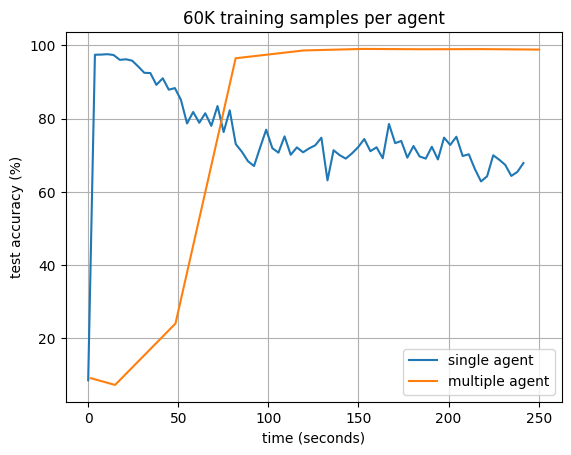
\includegraphics[width=\textwidth]{accuracy_60k}

To start off with, the swarm was a lot slower to increase its accuracy than the single agent algorithm, which is likely due to the higher overhead of running swarm learning. After some time, the swarm increased in accuracy to the same point as the single agent. However, after reaching this point, the single agent started to overfit but the swarm continued to increase in accuracy. The swam eventually settled upon a higher accuracy than the single agent ever achieved.

The agents seemed to reach the final accuracy in fewer training steps if the agents training loops were offset by even intervals of time. The author hypothesizes that this may be because when the agents training is synced, some of the agents may skip the just completed training when requesting updates, which can cause training epochs to effectively be lost. This effect needs further investigation.

\section{Reduced dataset swarm learning}
This experiment was focussed around reducing the amount of data each agent gets to train on. A number of samples were selected randomly for each agent from the training set, and these never changed throughout training. This test was run for 2000 and 500 samples per agent.

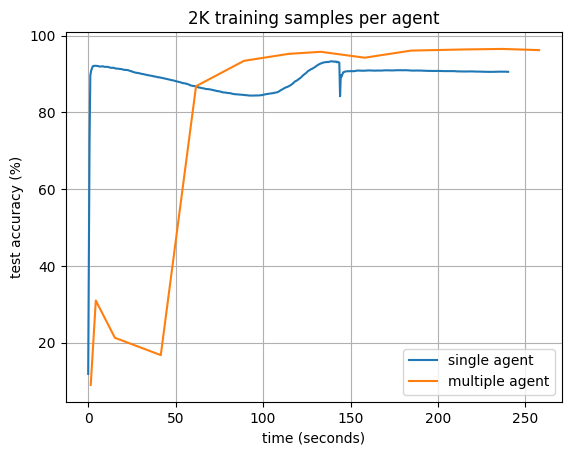
\includegraphics[width=\textwidth]{accuracy_2k}

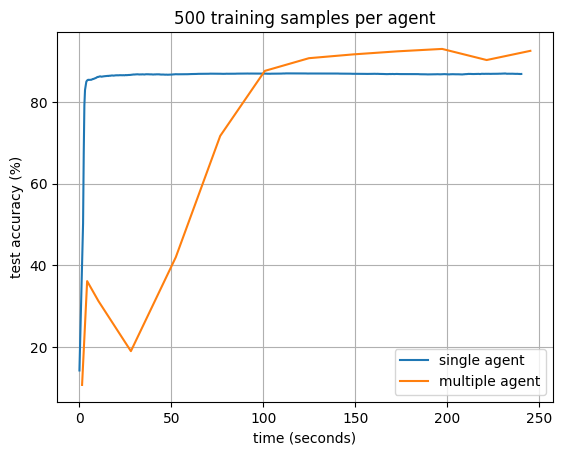
\includegraphics[width=\textwidth]{accuracy_500}

In both cases, the swarm took a lot longer to reach its peak accuracy, nevertheless, the swarm exceeded the peak accuracy of the lone agent by about 5\%-10\%.

On both graphs, there is a spike in accuracy near the start of swarm training, then a reduction in accuracy, then a stable increase. This is caused by new agents with untrained networks joining the swarm and adding effectively a random model to the pool of weights. An easy fix for this would to make an agent that has just joined the network request a model from its neighbours immediately, and use that as a base network. This has not been implemented due to time constraints. 